\chapter{Results and Analysis}
\label{ch:results}

This chapter presents the quantitative evaluation of each pipeline component and of the integrated system, following the protocol of Section~\ref{sec:eval_methodology}. Section~\ref{sec:res_perception} evaluates the perception module in and out of distribution. Section~\ref{sec:res_ablation} reports the depth-reconstruction ablation with statistical testing and the anchor-weight sweep. Section~\ref{sec:res_vla} presents the policy results, beginning with the diagnosis of a memorisation failure in the initial training configuration and proceeding to the corrected model's spatial accuracy, including an honest comparison against a positional-prior baseline. Section~\ref{sec:res_grasp} connects spatial accuracy to grasp feasibility, and Section~\ref{sec:res_latency} profiles runtime. Sections marked as placeholders await experiments in progress.

\section{Perception Module}
\label{sec:res_perception}

Table~\ref{tab:perception_results} summarises the perception module's surface-normal and segmentation accuracy. The in-distribution row is computed over the full \texttt{square-plastic-bottle} category (11{,}701 images) and therefore overlaps the network's training data; it should be read as an upper bound rather than a generalisation estimate. The two out-of-distribution (OOD) rows, computed on categories the network never observed, carry the generalisation claim.

\begin{table}[htbp]
    \centering
    \caption{Perception accuracy in and out of distribution. Angular errors in degrees over object pixels; threshold columns give the fraction of pixels with error below the stated angle. ID = in-distribution (overlaps training data); OOD = held-out category.}
    \label{tab:perception_results}
    \begin{tabular}{lcccccccc}
        \toprule
        \textbf{Category} & \textbf{Split} & \textbf{N} & \textbf{Mean} & \textbf{Median} & \textbf{RMSE} & \textbf{$<$11.25$^{\circ}$} & \textbf{$<$22.5$^{\circ}$} & \textbf{IoU} \\
        \midrule
        square-plastic-bottle & ID & 11{,}701 & 19.55$^{\circ}$ & 14.29$^{\circ}$ & 25.57$^{\circ}$ & 39.3\% & 69.4\% & 91.10\% \\
        cup-with-waves & OOD & 100 & 34.06$^{\circ}$ & 22.99$^{\circ}$ & 44.03$^{\circ}$ & 21.0\% & 49.1\% & 77.28\% \\
        champagne-glass & OOD & 117 & 25.53$^{\circ}$ & 18.00$^{\circ}$ & 33.71$^{\circ}$ & 27.8\% & 60.8\% & 77.87\% \\
        \bottomrule
    \end{tabular}
\end{table}

\begin{figure}[htbp]
    \centering
    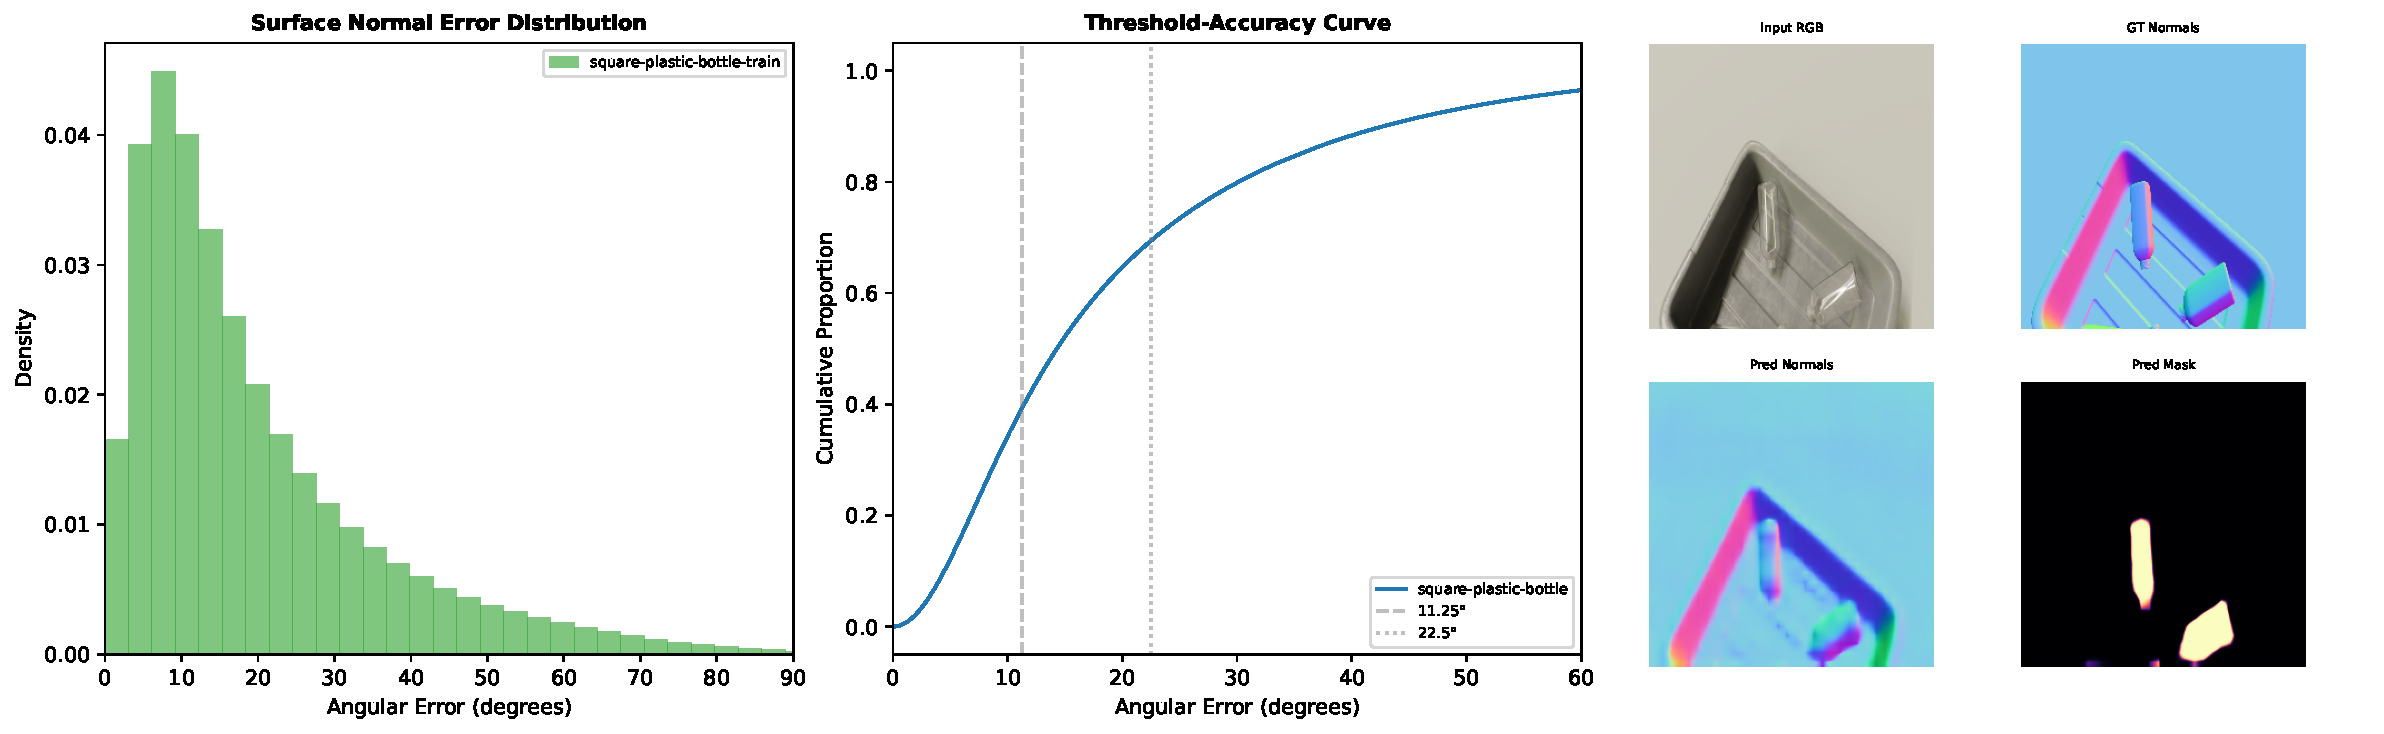
\includegraphics[width=\textwidth]{images/perception_evaluation_full.pdf}
    \caption{In-distribution perception behaviour on the training category. Left: surface-normal angular-error distribution, right-skewed with its mode near 8$^{\circ}$ and a long tail beyond 40$^{\circ}$. Centre: cumulative threshold-accuracy curve with the standard 11.25$^{\circ}$ and 22.5$^{\circ}$ thresholds marked. Right: a qualitative example (input RGB, ground-truth normals, predicted normals, predicted mask) showing accurate object localisation with smoothed normal detail. Out-of-distribution results are tabulated in Table~\ref{tab:perception_results}.}
    \label{fig:perception_full}
\end{figure}

The error distribution in Figure~\ref{fig:perception_full} is unimodal and right-skewed: most object pixels are estimated well (median 14.3$^{\circ}$), and the 19.55$^{\circ}$ mean is pulled upward by a minority of high-error pixels, concentrated---as the qualitative panel suggests---at object boundaries and internal refractive detail, where the prediction is visibly smoother than the ground truth.

Two further observations follow from Table~\ref{tab:perception_results}. First, segmentation generalises more gracefully than geometry: IoU falls by roughly 14 percentage points on unseen categories (91.1\% $\rightarrow$ $\sim$77.5\%), while mean angular error grows by between 31\% and 74\% depending on the target shape. The network still \emph{finds} unfamiliar transparent objects reliably but estimates their surface orientation less accurately. Second, the degradation is shape-dependent in a physically interpretable way: the stemless champagne glass---tall, smooth, and convex, geometrically similar to the training bottles---loses only 6$^{\circ}$ of mean accuracy, whereas the wavy-edged cup, whose corrugated surface has no analogue in the training data, loses 14.5$^{\circ}$. Generalisation appears to be governed by geometric similarity to the training category rather than by transparency per se.

\section{Depth Reconstruction Ablation}
\label{sec:res_ablation}

Table~\ref{tab:ablation_results} presents the four-way ablation over 100 images, with errors computed exclusively over the corrupted (transparent) region. Figure~\ref{fig:ablation_qualitative} shows representative reconstructions together with the per-method error distributions; Figure~\ref{fig:ablation_stats} isolates the mean RMSE with bootstrap confidence intervals.

\begin{table}[htbp]
    \centering
    \caption{Depth reconstruction error over the corrupted region (100 images, half resolution). Bootstrap 95\% confidence intervals from $10^{4}$ resamples.}
    \label{tab:ablation_results}
    \begin{tabular}{lccc}
        \toprule
        \textbf{Method} & \textbf{RMSE (m)} & \textbf{95\% CI} & \textbf{MAE (m)} \\
        \midrule
        (A) Raw corrupted depth & 0.9297 & [0.8646, 0.9965] & 0.9274 \\
        (B) Navier--Stokes inpainting & \textbf{0.1227} & [0.1152, 0.1306] & \textbf{0.1102} \\
        (C) Poisson + ground-truth normals & 0.1364 & [0.1250, 0.1490] & 0.1136 \\
        (D) Poisson + predicted normals & 0.4160 & [0.3936, 0.4390] & 0.2861 \\
        \bottomrule
    \end{tabular}
\end{table}

\begin{figure}[htbp]
    \centering
    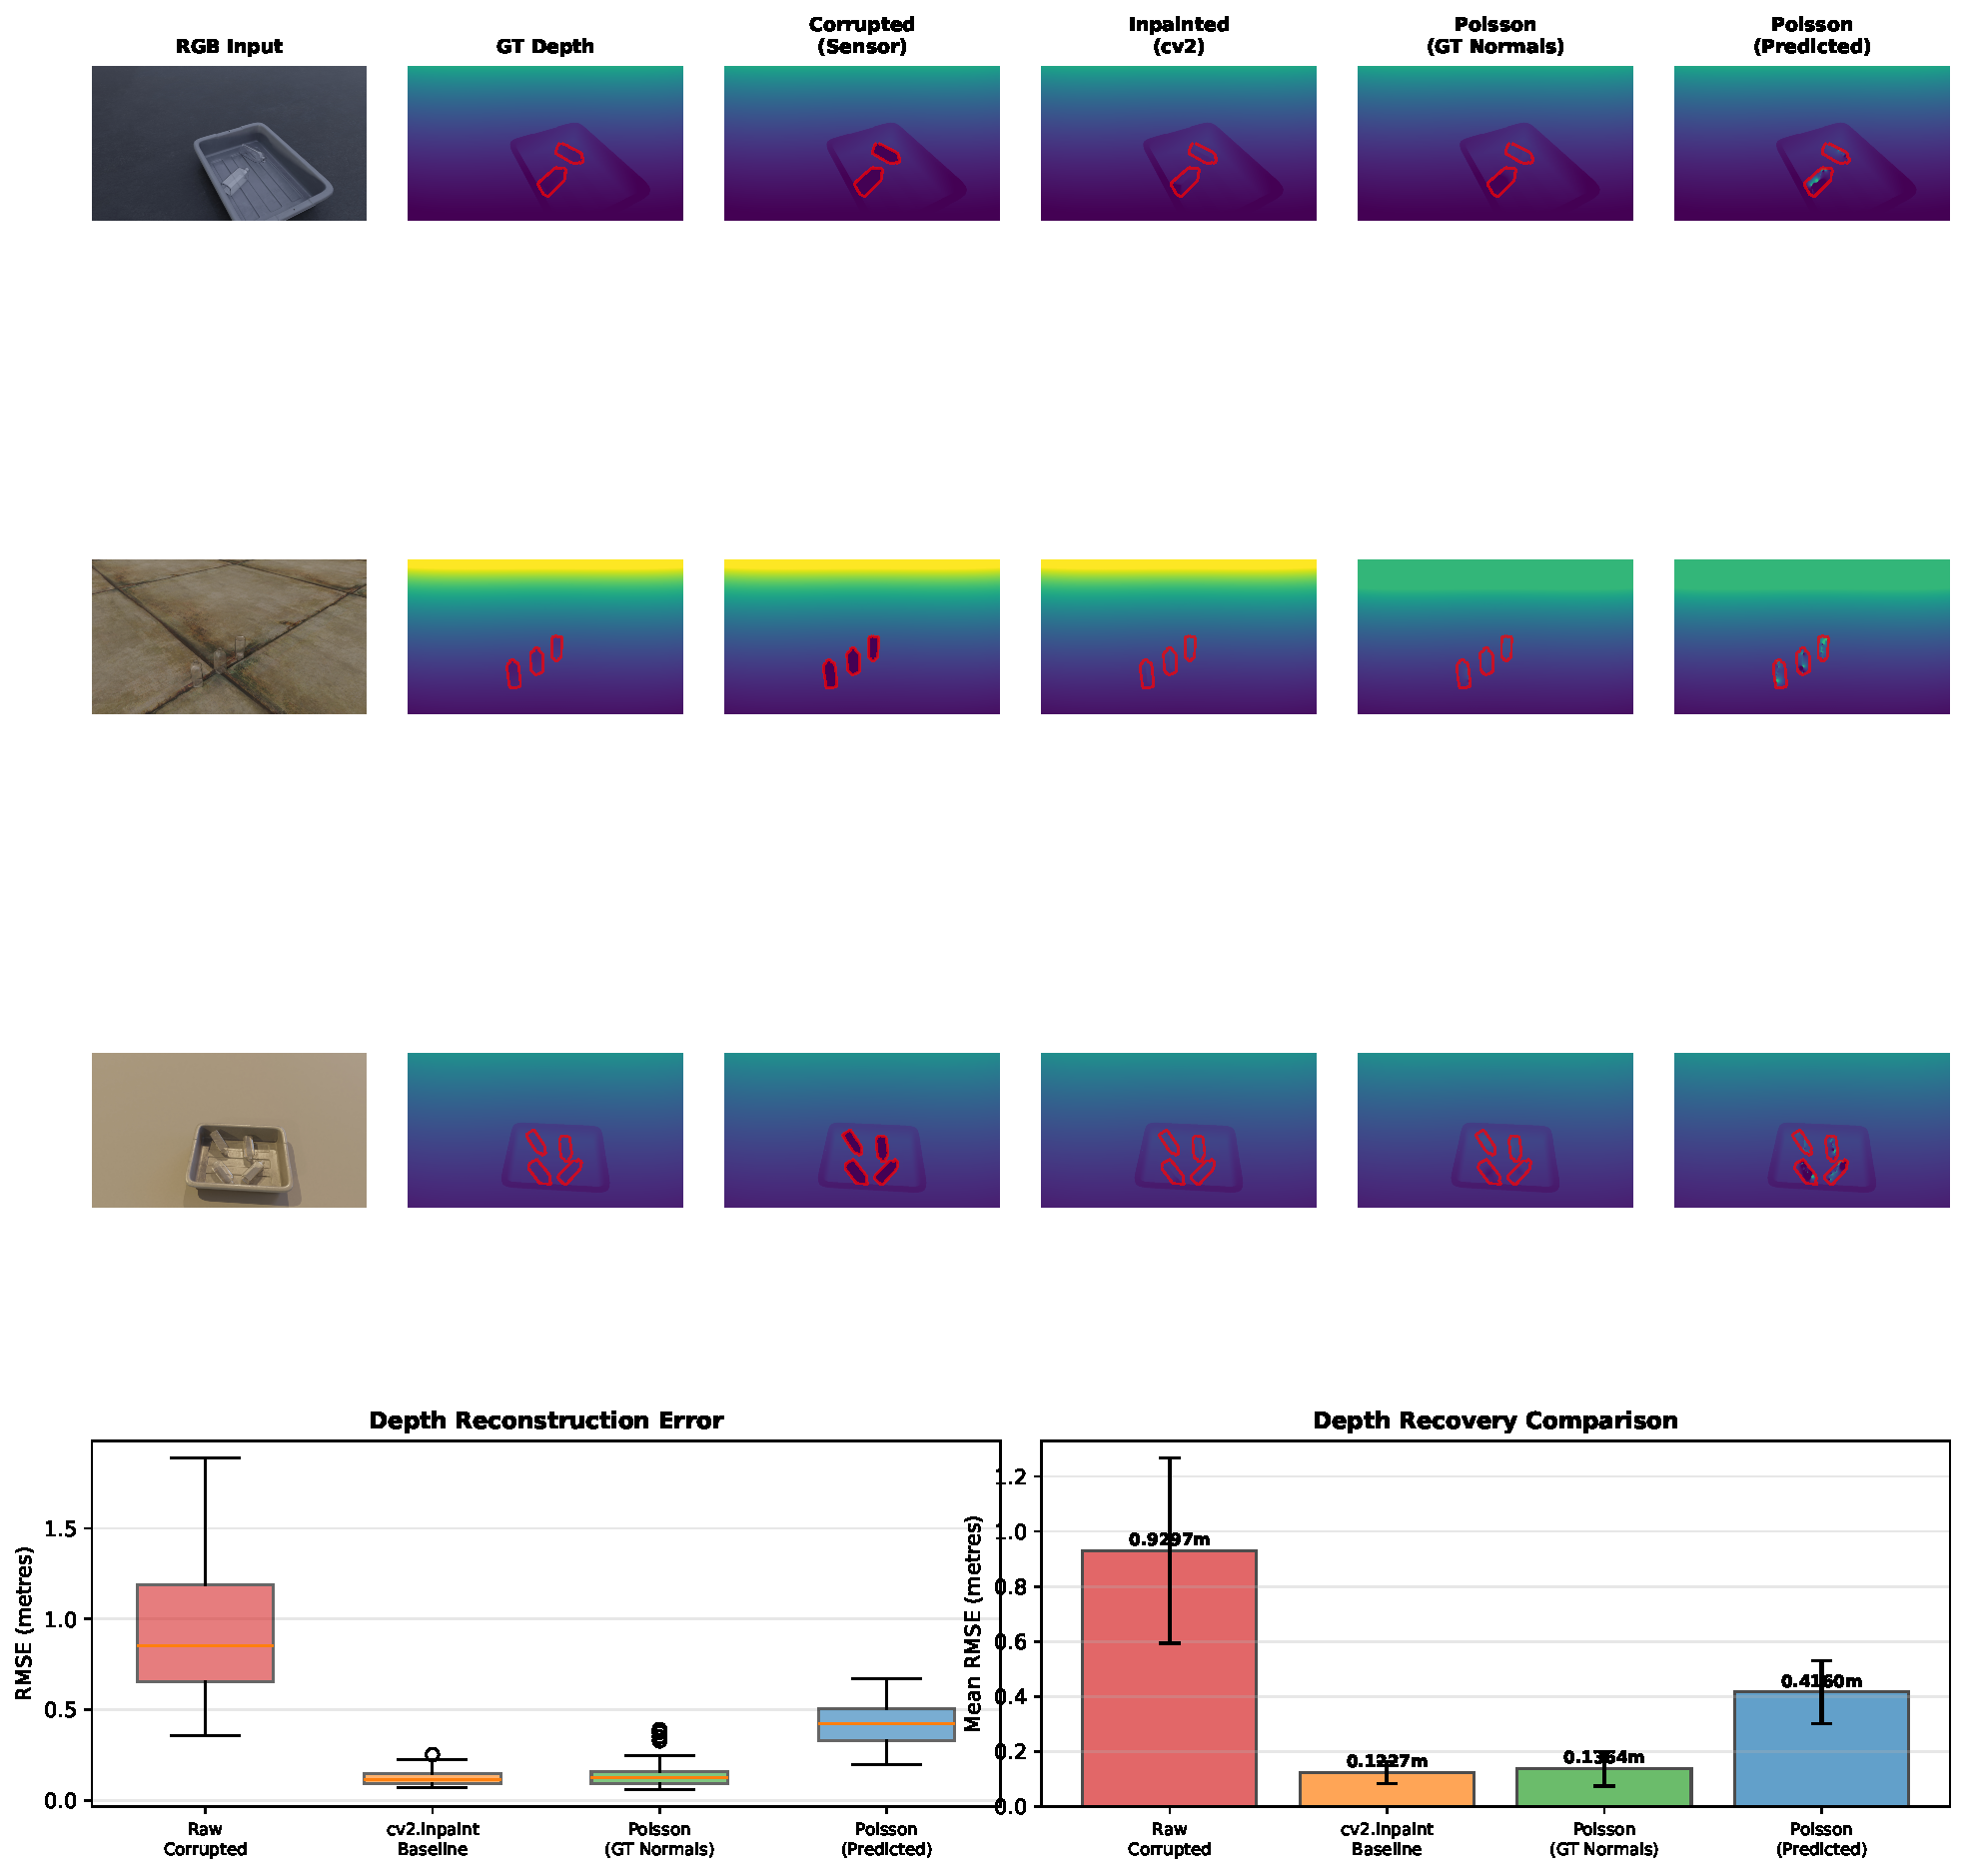
\includegraphics[width=\textwidth]{images/ablation_depth_reconstruction.pdf}
    \caption{Depth reconstruction ablation. Top rows: qualitative comparisons on three scenes (RGB input, ground-truth depth, corrupted sensor depth, inpainting baseline, Poisson with ground-truth normals, Poisson with predicted normals), with red contours marking the transparent regions; residual artefacts inside the contours are visible only in the predicted-normals condition. Bottom: RMSE box plots per method (note the outliers in the ground-truth-normals condition) and mean-RMSE bar chart.}
    \label{fig:ablation_qualitative}
\end{figure}

\begin{figure}[htbp]
    \centering
    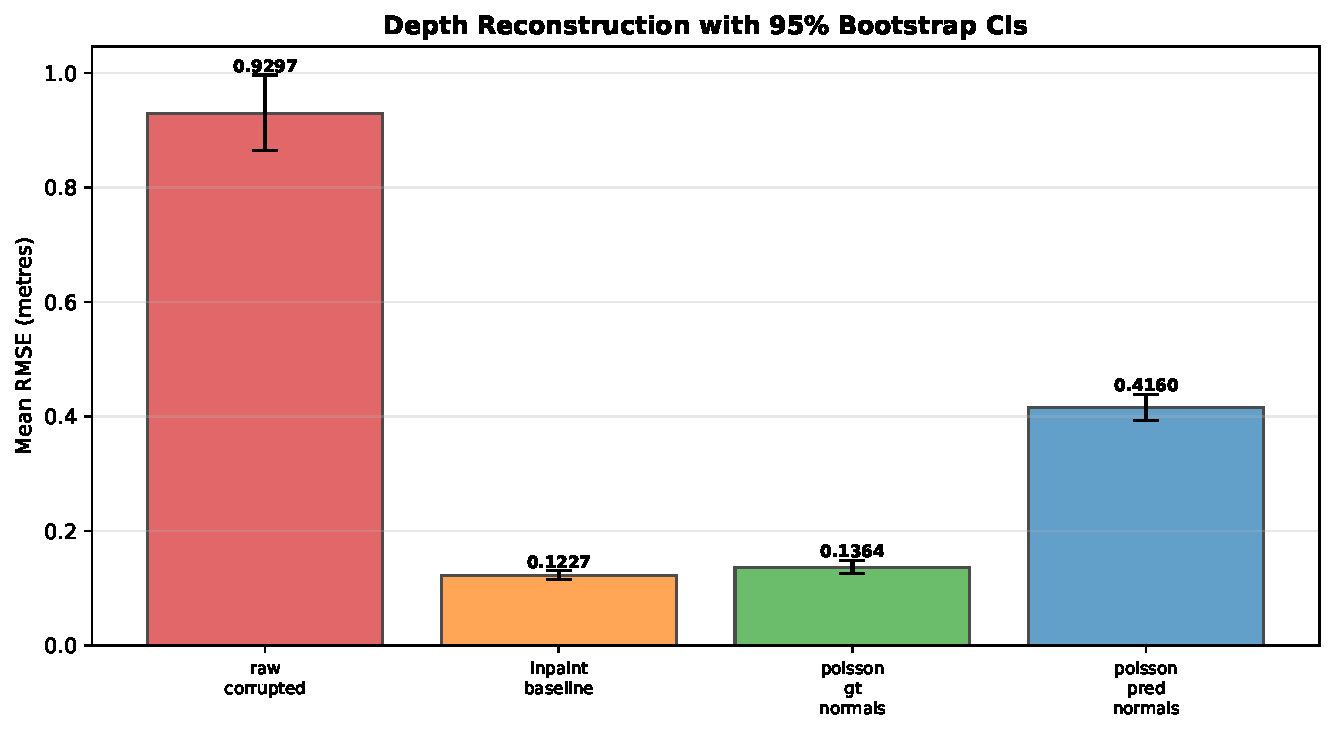
\includegraphics[width=0.8\textwidth]{images/ablation_statistics.pdf}
    \caption{Mean RMSE per reconstruction method with bootstrap 95\% confidence intervals. The intervals of the inpainting baseline and the ground-truth-normals solver overlap; the predicted-normals condition is separated from both by a wide margin.}
    \label{fig:ablation_stats}
\end{figure}

Paired Wilcoxon signed-rank tests over the matched images give the following comparisons. Both recovery methods improve enormously and significantly on the raw corrupted input (raw vs.\ inpainting: $p = 3.9 \times 10^{-18}$, median improvement $0.74$\,m). Between the two solvers, inpainting is marginally but significantly better than the Poisson solver driven by \emph{ground-truth} normals ($p = 0.02$, median difference $3.5$\,mm), and substantially better than the solver driven by \emph{predicted} normals ($p = 3.9 \times 10^{-18}$, median difference $0.29$\,m). The gap between conditions~C and~D isolates the cost of perception error: the same solver loses $0.28$\,m of RMSE when its normal input degrades from perfect to the 19.55$^{\circ}$ mean-error predictions of Section~\ref{sec:res_perception} ($p = 5.6 \times 10^{-18}$).

Two conclusions follow, one methodological and one architectural.
Methodologically, the near-parity of conditions~B and~C shows the solver is
implemented correctly---with perfect input it operates within 11\% of a strong
baseline---so condition~D's deficit is attributable to perception error, not
solver error. Architecturally, the result must be stated plainly: for the
object morphologies evaluated, geometry-unaware inpainting is not merely
competitive but statistically \emph{superior} to the Poisson solver even under
ground-truth normals ($p = 0.02$), while consuming a negligible fraction of
its runtime (Section~\ref{sec:res_latency} attributes 65\% of total pipeline
latency to the solver). The normal-guided reconstruction is therefore
unjustified for shallow, flat-lying objects such as the ClearGrasp bottles,
where boundary interpolation recovers essentially all of the depth field. This
is a scope boundary rather than a general invalidation---normal integration is
expected to earn its cost only where object depth varies substantially
relative to the surroundings (deep containers, stacked items)---but within the
present evaluation that expectation remains untested, and the honest
engineering conclusion is that the deployed configuration should use the
inpainting path.
\subsection{Anchor-Weight Sensitivity}
\label{subsec:res_lambda}

Table~\ref{tab:lambda_results} and Figure~\ref{fig:lambda} report the sensitivity of condition~C to the anchor weight $\lambda$ over a 30-image subset. Reconstruction error is stable to within 1.3\% across $\lambda \in [10, 100]$ and degrades beyond it (by 70\% at $\lambda = 500$ and 223\% at $\lambda = 1000$), where over-weighted anchors suppress the gradient constraints inside the hole. The operating value $\lambda = 100$ sits at the favourable end of the stable plateau; the method is therefore insensitive to this hyperparameter within an order of magnitude of the chosen value, and the choice was not tuned to the test data.

\begin{table}[htbp]
    \centering
    \caption{Reconstruction RMSE (condition C) as a function of anchor weight $\lambda$ (30 images).}
    \label{tab:lambda_results}
    \begin{tabular}{lccccc}
        \toprule
        $\lambda$ & 10 & 50 & 100 & 500 & 1000 \\
        \midrule
        RMSE (m) & 0.1277 & 0.1272 & \textbf{0.1260} & 0.2144 & 0.4069 \\
        Std (m) & 0.0489 & 0.0485 & 0.0433 & 0.0859 & 0.1330 \\
        \bottomrule
    \end{tabular}
\end{table}

\begin{figure}[htbp]
    \centering
    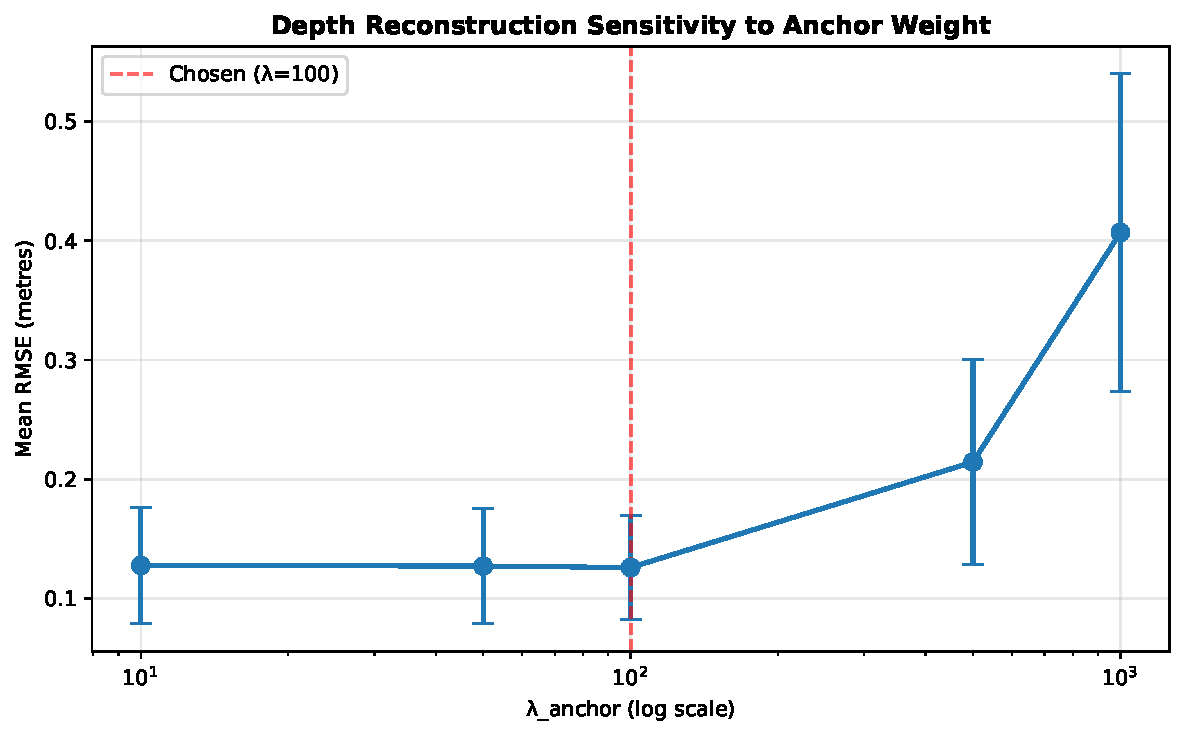
\includegraphics[width=0.7\textwidth]{images/lambda_sensitivity.pdf}
    \caption{Reconstruction RMSE against anchor weight $\lambda$ (log scale, error bars one standard deviation). The chosen operating point $\lambda = 100$ lies at the end of a flat plateau spanning $\lambda \in [10, 100]$.}
    \label{fig:lambda}
\end{figure}

\section{Policy Learning}
\label{sec:res_vla}

\subsection{Diagnosis of a Memorisation Failure}
\label{subsec:res_memorisation}

The initial fine-tuning configuration contained a data-pipeline defect: through a fault in the dataset loader, every training sample was paired with a single fixed action vector rather than its per-image grasp target. The resulting run is instructive precisely because its headline metrics looked excellent. Training loss fell from 26.08 to machine zero (0.0000) by step 4{,}480, and aggregate action-token accuracy on generation reached 97.71\%. Yet inspection of individual generations revealed that the model emitted an identical coordinate pair for every input image: it had memorised the constant label and learned nothing about the images. (A spatial error of 47 bins was recorded for this model, but by an evaluation script later found to mis-align the token slice; the figure is not directly comparable with the corrected measurements below and is not used quantitatively.)

This episode yields two generalisable observations. First, aggregate token accuracy is a misleading metric for VLA action strings in which most dimensions are constants: five of the seven action tokens here are fixed task parameters, so a policy that fails completely on the two informative coordinates can still score above 70\% by construction, and near-perfectly if it memorises the constants. Per-coordinate error must be reported separately. Second, a training loss reaching exactly zero is a diagnostic red flag rather than a success indicator---it certifies that the training set is memorisable, which for a spatial task implies the supervision lacks the diversity to force perceptual learning. These observations motivated the loss masking, per-sample target verification, and continuous validation monitoring of Section~\ref{subsec:training_protocol}.

\subsection{Corrected Training Dynamics}
\label{subsec:res_training}

With per-image targets, background-identity splitting, and the augmentation suite of Section~\ref{subsec:compositing} in place, the training dynamics changed qualitatively. Loss fell from 25.4 and plateaued near 0.15--0.17 without approaching zero; validation loss tracked training loss closely throughout, indicating that the residual error reflects task difficulty rather than overfitting. Early stopping halted training at step 21{,}500 (mid-second-epoch) with a best validation loss of 0.154. A preliminary corrected run at double the learning rate ($2 \times 10^{-5}$) with a tighter patience of 5 stopped much earlier (step 7{,}800) at a statistically indistinguishable validation loss, indicating that the model reaches a data-limited ceiling quickly: the remaining error is bounded by the data, not the training budget.

\subsection{Spatial Accuracy}
\label{subsec:res_spatial}
 
Policy accuracy was evaluated by autoregressive generation on held-out
validation composites across all saved checkpoints (50 samples per
checkpoint; checkpoints whose generations produced more than five unparseable
outputs are excluded from trend analysis, as parser contamination inflates
their per-axis means). Table~\ref{tab:vla_comparison} compares the spatial
accuracy of the two training iterations, and
Figure~\ref{fig:vla_checkpoints_run2} shows the learning trajectory of the
second run.
 
\begin{table}[htbp]
    \centering
    \caption{VLA spatial accuracy across the two training iterations.
    Clean checkpoints only (parse failures $\leq 5$).}
    \label{tab:vla_comparison}
    \begin{tabular}{lcc}
        \toprule
        & \textbf{Run 1} & \textbf{Run 2} \\
        \midrule
        Training data & composites only (640$\times$480) & 50/50 composite + native (224$\times$224) \\
        Label validity & 90.0\% & 100\% \\
        Dataset size & 24{,}570 train & 30{,}850 train \\
        Best-checkpoint L1 (bins) & 27.60 & 20.59 \\
        Best-checkpoint median L1 & 26.50 & 21.00 \\
        X error (bins) & 32.70 & 23.98 \\
        Y error (bins) & 32.46 & 27.47 \\
        \bottomrule
    \end{tabular}
\end{table}
 
The best clean checkpoint of the second run (step 20{,}500) achieves a mean
spatial L1 error of \textbf{20.59 bins} (median 21.0), with per-axis
coordinate errors of 23.98 (x) and 27.47 (y). This represents a 25\%
reduction in mean L1 error relative to the first run's best (27.60 bins).
Multiple nearby checkpoints perform comparably (steps 16{,}000, 22{,}000,
22{,}500, 30{,}500 all fall in the 21--22 bin range), indicating a stable
convergence plateau rather than a lucky single checkpoint.
 
\begin{figure}[htbp]
    \centering
    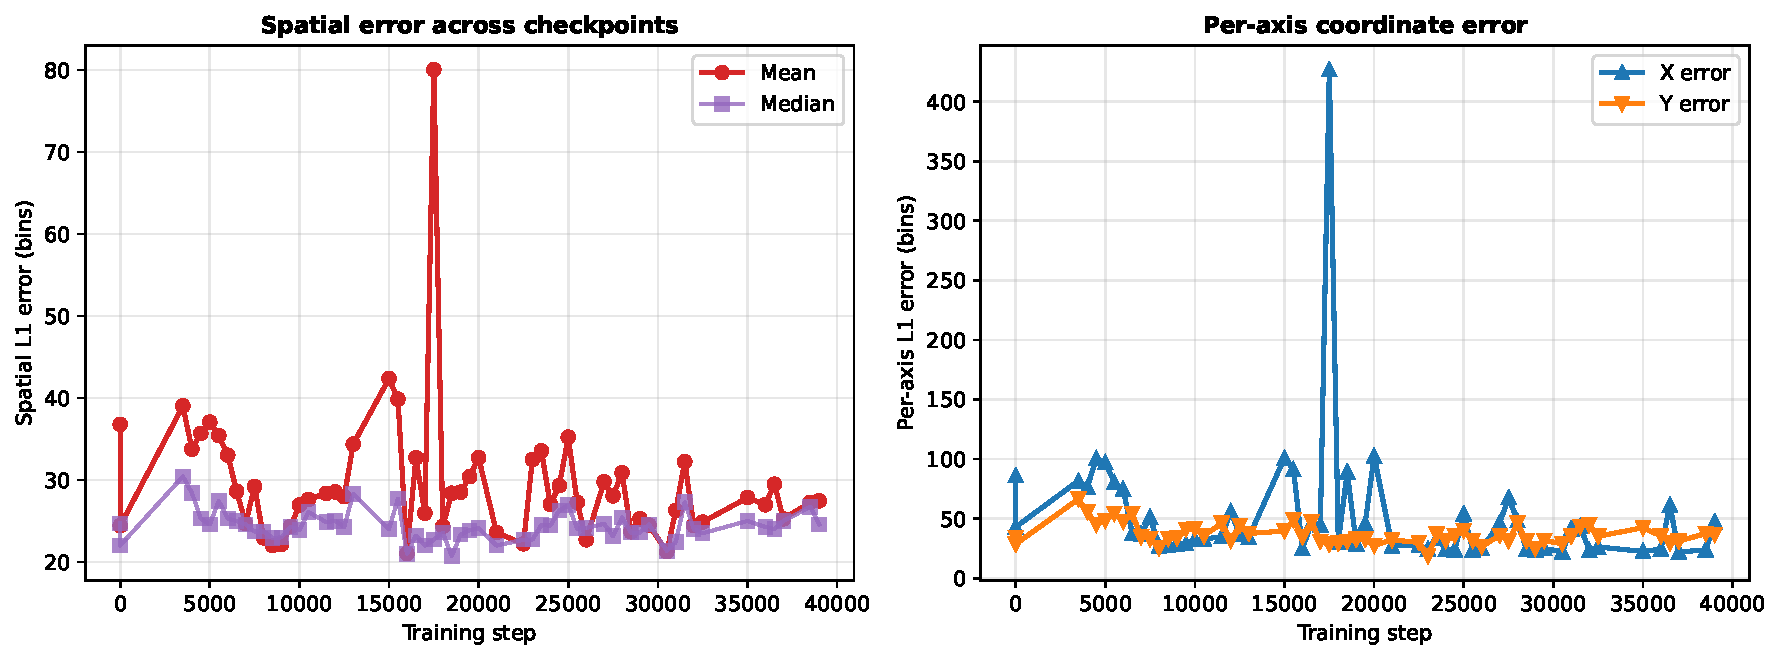
\includegraphics[width=\textwidth]{images/vla_checkpoint_curves2.pdf}
    \caption{Run~2 spatial L1 error (left: mean and median) and per-axis
    coordinate error (right) across training checkpoints. The mean is
    volatile due to parser contamination at some checkpoints; the median
    (purple) is stable and falls to $\sim$21 bins by step 8{,}000,
    remaining there through 39{,}000 steps.}
    \label{fig:vla_checkpoints_run2}
\end{figure}
 
The per-axis asymmetry (X $\approx$ 24, Y $\approx$ 27--45 across
checkpoints) warrants comment. The Y error is consistently higher and more
variable than X, which may reflect the vertical composition bias of the
ClearGrasp renders (objects typically sit in the lower portion of the frame)
combined with the reduced vertical extent of objects at 224$\times$224.
 

 
\section{Grasp-Feasibility Measurement}
\label{sec:res_grasp}
 
\subsection{Label Audit}
\label{subsec:res_labelaudit}
 
An exact mask-based evaluation of the first training iteration exposed a
defect in the training labels themselves: only 90.0\% of ground-truth targets
lay inside their target mask (171/190). The cause is geometric---for concave
or crescent-shaped objects, the contour centroid used for target derivation
falls outside the object boundary---and the consequence is that approximately
one in ten training samples across all 24{,}570 composites supervised the
policy to target empty background. This label noise both contaminated
training and deflated the measured success rates. Its correction
(point-in-polygon validation with a distance-transform fallback,
Section~\ref{subsec:target_derivation}) is one of the three data revisions of
the second training iteration, which achieves 100\% label validity by
construction.
 
\subsection{Run~1 Baseline}
\label{subsec:res_grasp_run1}
 
Under exact mask evaluation, the first-generation model (190 parseable
validation samples) achieves: \textsc{on-target} 2.6\% (Wilson 95\% CI
[1.1\%, 6.0\%]), \textsc{on-object} 4.7\% ([2.5\%, 8.8\%]), and
\textsc{proximity} (40\,px) 14.7\% ([10.4\%, 20.5\%]). The comparison
between criteria is itself informative: the proximity figure, initially
interpreted as a conservative lower bound, is in fact an optimistic upper
bound---most predictions within the 40-pixel disc land on background pixels
adjacent to the object, not on the object itself. The plain statement is that
the first-generation policy fails to place its target on solid object
material in more than 97\% of cases.
 
\subsection{Run~2: Effect of Data Revisions}
\label{subsec:res_grasp_run2}
 
Three root-cause revisions were applied and the policy retrained from
scratch: (i)~validity-guaranteed targets ($10\% \rightarrow 0\%$ label
noise); (ii)~a 50/50 mixture of composites and native ClearGrasp frames; and
(iii)~generation at the encoder-native $224 \times 224$ resolution.
Table~\ref{tab:run_comparison} compares the two runs under identical
mask-exact evaluation.
 
\begin{table}[htbp]
    \centering
    \caption{Grasp-feasibility comparison between training iterations under
    identical mask-exact evaluation. Wilson 95\% confidence intervals in
    brackets.}
    \label{tab:run_comparison}
    \begin{tabular}{lcc}
        \toprule
        & \textbf{Run 1} ($n = 190$) & \textbf{Run 2} ($n = 251$) \\
        \midrule
        Label validity & 90.0\% & 100\% \\
        Training mix & composites only & 47\% composite / 53\% native \\
        Resolution & $640{\times}480 \rightarrow 224$ & native $224{\times}224$ \\
        Mean spatial L1 (bins) & 27.6 & 20.6 \\
        \midrule
        \textsc{on-target} & 2.6\% [1.1, 6.0] & \textbf{7.2\%} [4.6, 11.0] \\
        \textsc{on-object} & 4.7\% [2.5, 8.8] & \textbf{12.7\%} [9.2, 17.4] \\
        \bottomrule
    \end{tabular}
\end{table}
 
On-target rate nearly tripled (2.6\% $\rightarrow$ 7.2\%) and on-object rate
nearly tripled (4.7\% $\rightarrow$ 12.7\%). While these remain far below
deployment-grade precision, the improvement is statistically significant: the
Run~2 on-object confidence interval [9.2\%, 17.4\%] does not overlap with
the Run~1 interval [2.5\%, 8.8\%].
 
\subsection{Breakdown by Sample Type}
\label{subsec:res_grasp_type}
 
The most diagnostic finding of this evaluation is the performance split
between native ClearGrasp frames and composites within the Run~2 validation
set (Table~\ref{tab:grasp_by_type}).
 
\begin{table}[htbp]
    \centering
    \caption{Run~2 grasp accuracy by sample type. Wilson 95\% CIs in brackets.}
    \label{tab:grasp_by_type}
    \begin{tabular}{lccc}
        \toprule
        \textbf{Sample type} & $n$ & \textbf{\textsc{on-target}} & \textbf{\textsc{on-object}} \\
        \midrule
        Native ClearGrasp & 124 & \textbf{11.3\%} [6.8, 18.1] & \textbf{20.2\%} [14.0, 28.1] \\
        Composite          & 127 & 3.1\% [1.2, 7.8] & 5.5\% [2.7, 10.9] \\
        \bottomrule
    \end{tabular}
\end{table}
 
The model is nearly four times more accurate on native frames (11.3\%
on-target) than on composites (3.1\%). This directly confirms the hypothesis
of Section~\ref{subsec:realframe_mixing}: compositing removes the
transparency-specific cues---refraction, shadows, specular highlights---that
carry spatial information for transparent objects, and restoring those cues
via real renders measurably improves localisation. The composite performance
in Run~2 (3.1\%) is comparable to the full-dataset performance of Run~1
(2.6\%), indicating that the Run~2 improvement is attributable almost
entirely to the native-frame component of the training mix rather than to the
label or resolution fixes alone.
 
\subsection{Breakdown by Object Size}
\label{subsec:res_grasp_size}
 
Table~\ref{tab:grasp_by_size} reports grasp accuracy across object-area
terciles. The pattern is unambiguous: the model cannot localise small objects
at all (0\% on-target), achieves marginal accuracy on medium objects (7.3\%),
and its best performance on large objects (14.1\% on-target, 20.0\%
on-object). At the $224 \times 224$ working resolution, ``small'' objects
occupy fewer than 142 pixels of area---a footprint too limited to resolve at
the VLA encoder's patch granularity.
 
\begin{table}[htbp]
    \centering
    \caption{Run~2 grasp accuracy by object-area tercile. Wilson 95\% CIs in brackets.}
    \label{tab:grasp_by_size}
    \begin{tabular}{lcccc}
        \toprule
        \textbf{Size band} & $n$ & \textbf{\textsc{on-target}} & \textbf{\textsc{on-object}} \\
        \midrule
        Small ($< 142$\,px)  &  84 & 0.0\% [0.0, 4.4] & 2.4\% [0.7, 8.3] \\
        Medium               &  82 & 7.3\% [3.4, 15.1] & 15.9\% [9.5, 25.3] \\
        Large ($\geq 562$\,px) & 85 & \textbf{14.1\%} [8.3, 23.1] & \textbf{20.0\%} [12.9, 29.7] \\
        \bottomrule
    \end{tabular}
\end{table}
 
\begin{figure}[htbp]
    \centering
    
\includegraphics[width=\textwidth]{images/grasp_success_gallery_run2.pdf}
    \caption{Run~2 grasp-target predictions. Left two: \textsc{target hit}
    (prediction on the selected object---note the tote context with real
    shadows). Middle two: \textsc{other object} (prediction on a different
    item in the cluster). Right two: \textsc{miss} (prediction on background).
    Yellow contours: target object; cyan contours: all objects; red cross:
    prediction; green cross: ground truth.}
    \label{fig:grasp_gallery_run2}
\end{figure}
 
 
% ────────────────────────────────────────────────────────────────────────────
% CHAPTER 4 §4.9 — REPLACE the Summary of Findings
% ────────────────────────────────────────────────────────────────────────────
 
\section{Summary of Findings}
\label{sec:res_summary}
 
Against the research questions: the perception module recovers
transparent-object geometry with 19.6$^{\circ}$ mean normal error in
distribution, degrading gracefully and shape-dependently out of distribution
while segmentation remains robust (RQ2). Normal-guided depth reconstruction
matches a strong inpainting baseline when given perfect normals; for the
shallow object geometries evaluated, geometry-unaware inpainting is not
merely competitive but statistically superior, while the 0.28\,m gap between
perfect and predicted normals cleanly quantifies perception-to-depth error
propagation (RQ3).
 
Two training iterations characterise the VLA's spatial-grounding capacity on
synthetic data (RQ1). The first, trained on composites only with 10\% invalid
labels, yielded a model whose mean precision did not exceed a positional
prior and whose predictions landed on object material in under 3\% of cases.
The second---with corrected labels, native resolution, and a 50/50
native/composite mix---nearly tripled the on-target rate to 7.2\% and
reduced mean spatial error by 25\%, with a striking type breakdown: 11.3\%
on-target on native frames versus 3.1\% on composites, directly confirming
compositing fidelity as the dominant bottleneck. A clear size effect (0\% on
small objects, 14.1\% on large) identifies encoder resolution as a secondary
constraint. Throughput is 0.26\,FPS, bounded by the CPU depth solver (65\%)
rather than the language model (RQ4).
 
\section{End-to-End Qualitative Results}
\label{sec:res_e2e}

Figure~\ref{fig:pipeline_gallery} traces the full pipeline on four native ClearGrasp scenes: RGB observation, predicted surface normals, reconstructed metric depth, and the VLA's grasp target overlaid with the object boundaries. Two points about this gallery deserve emphasis. First, the perception-to-depth path is visually convincing: normals localise the transparent objects and the reconstructed depth is plausible across tote and floor scenes. Second, these images constitute a \emph{domain shift for the policy}, which was trained on ReSort-IT composites rather than native renders; its targets here land near, but frequently not on, the intended objects (upper rows), consistent with---and if anything slightly worse than---the in-domain quantitative results of Section~\ref{sec:res_grasp}. The gallery therefore doubles as an informal robustness probe.

\begin{figure}[htbp]
    \centering
    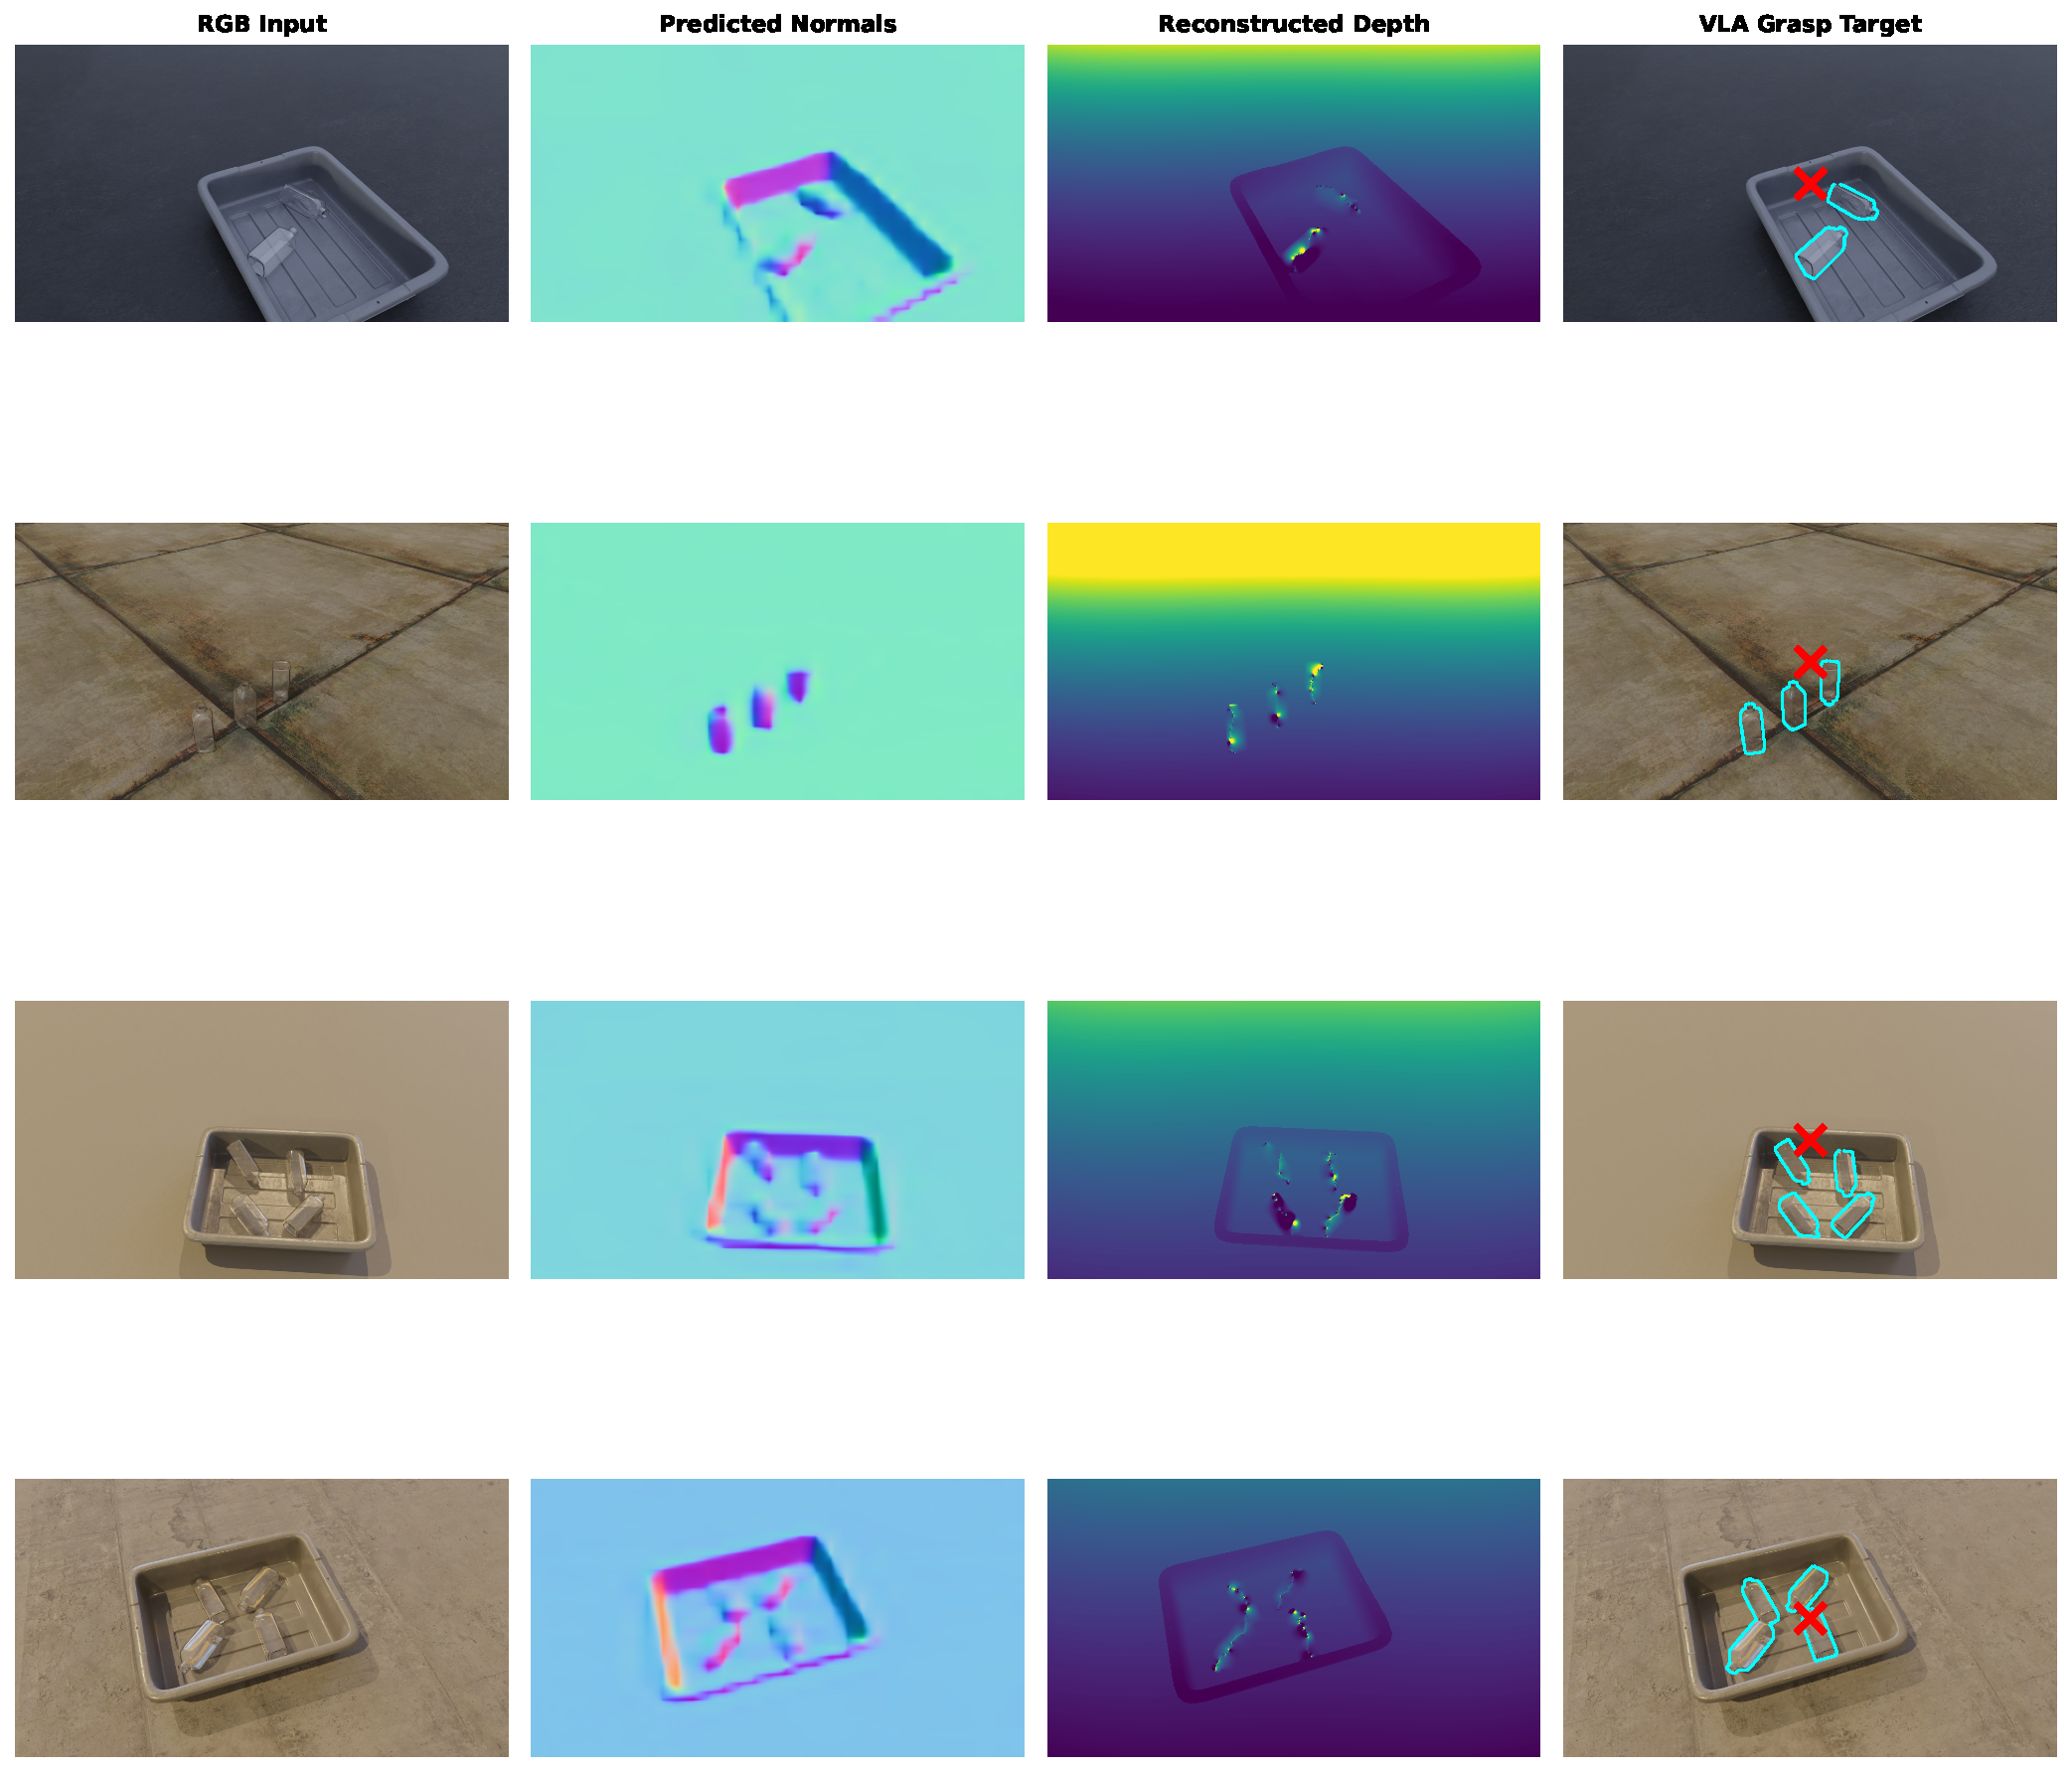
\includegraphics[width=\textwidth]{images/pipeline_gallery.pdf}
    \caption{End-to-end pipeline outputs on four native ClearGrasp scenes (a domain shift from the policy's composite training data). Columns: RGB input, predicted normals, reconstructed depth, VLA grasp target (red cross) with object boundaries (cyan).}
    \label{fig:pipeline_gallery}
\end{figure}

\section{Semantic Reasoning Evaluation}
\label{sec:res_semantic}

The model followed the category-specific instruction in 34 of 55 valid paired comparisons (61.8%), above the 50% baseline of an instruction-blind model but not statistically significant at the 95% level (Wilson CI [48.6%, 73.5%]). Inspection of individual scenes reveals bimodal behaviour: in approximately 40% of cases, the prediction shifts meaningfully toward the named object. In the remaining scenes, the model produces near-identical predictions regardless of the instruction. Qualitative visual analysis suggests this static behaviour frequently occurs when transparent targets are obscured by high-contrast adversarial backgrounds, indicating that language conditioning collapses when visual feature extraction fails.

Furthermore, the model suffered 17 parsing failures, generating invalid token syntax when presented with out-of-distribution prompts. Together, this pattern suggests that LoRA fine-tuning on a single instruction template partially degraded the pretrained language conditioning and syntax generation of the frozen backbone—a finding consistent with the catastrophic forgetting literature. Training on diverse instruction templates and visually clearer baseline backgrounds is the indicated remedy for future semantic-reasoning work.
\begin{figure*}[h!]
    \centering
    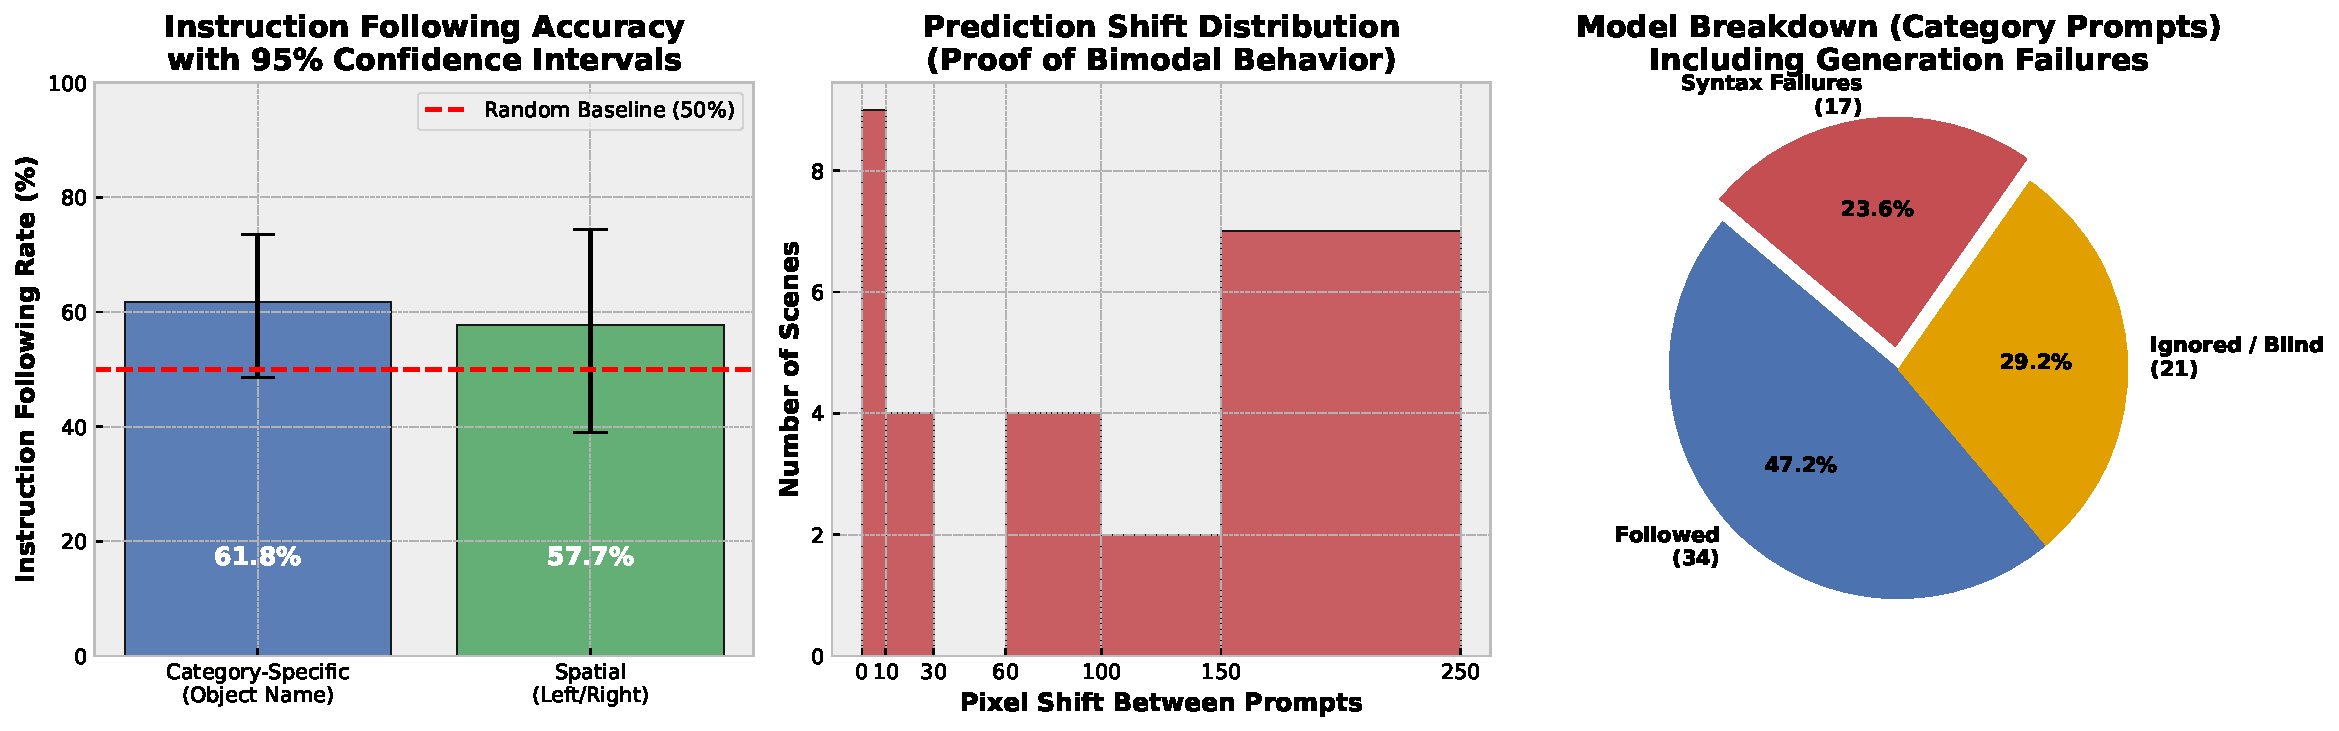
\includegraphics[width=\textwidth]{images/semantic_evaluation_graphs.pdf}
    \caption{Zero-shot semantic reasoning evaluation. (Left) Instruction following accuracy with 95\% Wilson confidence intervals compared to a 50\% random baseline. (Center) Pixel shift distribution between identical scenes given differing prompts, highlighting bimodal behaviour. (Right) Global breakdown of prompt responses, indicating severe language generation degradation (syntax failures).}
    \label{fig:semantic_eval}
\end{figure*}


\section{Simulation Integration}
\label{sec:res_gazebo}

\textbf{[PLACEHOLDER --- OPTIONAL, TIME-PERMITTING: Gazebo integration of the ABB IRB 360 with the pipeline's 3D targets. If the timeboxed attempt succeeds, insert setup description, a figure of the simulated cell, and pick-execution observations. Otherwise DELETE THIS SECTION and retain simulation as future work in Chapter~6.]}

\section{Summary of Findings}
\label{sec:res_summary}

Against the research questions: the perception module recovers transparent-object geometry with 19.6$^{\circ}$ mean normal error in distribution, degrading gracefully and shape-dependently out of distribution while segmentation remains robust (RQ2). Normal-guided depth reconstruction matches a strong inpainting baseline when given perfect normals, and the measured 0.28\,m gap between perfect and predicted normals cleanly quantifies perception-to-depth error propagation; for the shallow object geometries evaluated, geometry-unaware inpainting is competitive (RQ3). 
The first training iteration establishes the failure modes with precision:
composites-only supervision, contaminated by 10\% invalid labels and stripped
of transparency-specific localisation cues, produced a policy whose mean
precision does not exceed the dataset's positional prior and whose predictions
land on object material in under 3\% of cases. Each identified cause was
corrected in a second iteration---validity-guaranteed labels, a 50/50 native/
composite mix, and encoder-native resolution---whose results
(Section~\ref{subsec:res_run2}) determine how much of the failure is
attributable to data fidelity as opposed to the architecture itself (RQ1,
RQ4). Throughput is 0.26\,FPS, bounded by the CPU depth solver 
rather than the language model (RQ4).